\documentclass[12pt]{article}
\usepackage[utf8]{inputenc}
\usepackage[english]{babel}
\usepackage{listings}
\usepackage{tikz}
\usepackage{amsmath,amssymb}
\tikzset{main node/.style={circle,fill=white!20,draw,minimum size=1cm,inner sep=0pt},}
\usepackage{verbatim}
\newcommand{\HRule}{\rule{\linewidth}{0.5mm}}

\begin{document}

\begin{center}
\textsc{\LARGE Principles of Computer System Design}\\[0.3cm] % Context
\HRule \\[0.4cm]
{ \huge \bfseries Assignment 2} % Main title
\HRule \\[0.4cm]
\large
Johannes de Fine Licht % Names
\\Philip Graae
\\Ola Rønning
\\\today
\end{center}

\section*{Question 1: Serializability \& Locking} % Question 1

\subsection*{Schedule 1}
\begin{figure}[h!]
\texttt{T1: R(X)\hspace{250pt}W(Y) C\\
T2:\hspace{50pt}W(Z) W(X) C \\
T3:\hspace{150pt}R(Z) R(Y) C}
\caption{Schedule one.}
\label{sch1}
\end{figure}
Schedule one, reproduced above, correspondence to the precedence graph in figure~\ref{p1}.
\begin{figure}[h!]
\centering
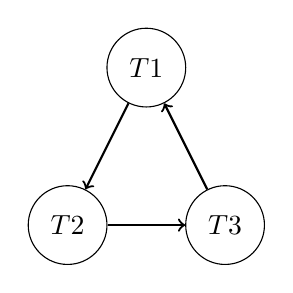
\begin{tikzpicture}
    \node[main node] (1) at (0,1)      {$T1$};
    \node[main node] (2) at (-1, -1) {$T2$};
    \node[main node] (3) at (1, -1)  {$T3$};

    \path[draw,thick,->]
    (1) edge node {} (2)
    (2) edge node {} (3)
    (3) edge node {} (1);
\end{tikzpicture}
\caption{Precedence graph for Schedule one, see figure~\ref{sch1}.}
\label{p1}
\end{figure}
The precedence graph, see figure~\ref{p1}, contains a cycle between transactions: \texttt{T1,T2,T3} and is hence not conflict serializable. As schedulers using Strict two phase locking allows only conflict serializable schedules. Schedule one is not conflict serializable and therefore cannot have been produced by a scheduler following Strict two phase locking.
\subsection*{Schedule 2} 
\begin{figure}[h!]
\texttt{T1: R(X)\hspace{150pt}W(Y) C\\
T2:\hspace{130pt}R(Z)\hspace{120pt}W(X) W(Y) C\\
T3:\hspace{50pt}W(Z) C}
\caption{Schedule two.}
\label{sch2}
\end{figure}
Schedule two, reproduced above, correspondence to the precedence graph in figure~\ref{p2}.
\begin{figure}[h!]
\centering
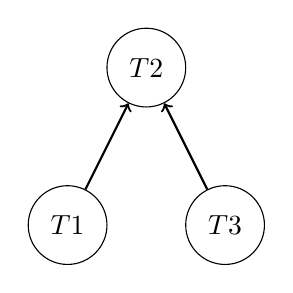
\begin{tikzpicture}
    \node[main node] (2) at (0,1)    {$T2$};
    \node[main node] (1) at (-1, -1) {$T1$};
    \node[main node] (3) at (1, -1)  {$T3$};

    \path[draw,thick,->]
    (1) edge node {} (2)
    (3) edge node {} (2);
\end{tikzpicture}
\caption{Precedence graph for Schedule one, see figure~\ref{sch2}.}
\label{p2}
\end{figure}
The precedence graph, see figure~\ref{p2}, is acyclic and hence is conflict serializable. In particular schedule two, is equivalent with a serial schedule where transaction two is performed last. As schedule 2 is conflict serializable, schedule 2 could be scheduled by a scheduler following Strict two phase locking. The injection of shared and exclusive locks required if the scheduler was using Strict two phase locking is reproduced below, figure~\ref{locks}.
\begin{figure}[h!]
\texttt{T1: S(X)\hspace{95pt}E(Y)RS(X)RE(Y)\\
T2:\hspace{105pt}S(Z)\hspace{90pt}E(X)E(Y)RS(Z)RE(X)RE(Y)\\
T3:\hspace{50pt}E(Z)RE(Z)}
\label{locks}
\caption{Shared and exclusive locks that need to be acquired in order for schedule two, see figure~\ref{sch2}, to be scheduled using Strict two phase locking. \texttt{S(Q)} acquires a shared lock on \texttt{Q} and \texttt{RS(Q)} releases the lock on \texttt{Q}, exclusive locks follow the same semantics, only with an \texttt{E}.}
\end{figure}
\section*{Question 2: Optimistic Concurrency Control}
\subsection*{Scenario 1}
\begin{figure}[h!]
\texttt{T1: RS(T1) = \{1, 2, 3\}, WS(T1) = \{3\},\\
T1 completes before T3 starts.\\
T2: RS(T2) = \{2, 3, 4\}, WS(T2) = \{4, 5\},\\
T2 completes before T3 begins with its write phase.\\
T3: RS(T3) = \{3, 4, 6\}, WS(T3) = \{3\},\\
allow commit or rollback?}
\caption{Scenario one.}
\label{sc1}
\end{figure}
In scenario one, see figure~\ref{sc1}, will have to rollback because of the offending object \texttt{4} in the write set of transaction two and the read set of transaction three. The conflict occurs because transaction two completes before transactions threes begins its write phase, and the intersection of their sets are non-empty.
\begin{align}
WS(T2) \cap RS(T3) &= \{4, 5\} \cap \{3, 4, 5\}\\
&= \{4\} \neq \emptyset
\end{align}
\subsection*{Scenario 2}
\begin{figure}[h!]
\texttt{T1: RS(T1) = \{2, 3, 4, 5\}, WS(T1) = \{4\},\\
T1 completes before T3 begins with its write phase.\\
T2: RS(T2) = \{6, 7, 8\}, WS(T2) = \{6\},\\
T2 completes read phase before T3 does.\\
T3: RS(T3) = \{2, 3, 5, 7, 8\}, WS(T3) = \{7, 8\},\\
allow commit or rollback?}
\caption{Scenario two.}
\label{sc2}
\end{figure}
In scenario two, see figure~\ref{sc2}, will have to rollback of the offending object \texttt{3} in the write set of transaction one and the read set of transaction three. The conflict occurs because transaction one completes before transactions threes begins its write phase, and the intersection of their sets are non-empty.
\begin{align}
WS(T1) \cap RS(T3) &= \{3\} \cap \{3, 4, 5, 6, 7\}\\
&= \{3\} \neq \emptyset
\end{align}
\subsection*{Scenario 3}
\begin{figure}[h!]
\texttt{T1: RS(T1) = \{2, 3, 4, 5\}, WS(T1) = \{4\},\\
T1 completes before T3 begins with its write phase.\\
T2: RS(T2) = \{6, 7, 8\}, WS(T2) = \{6\},\\
T2 completes before T3 begins with its write phase.\\
T3: RS(T3) = \{2, 3, 5, 7, 8\}, WS(T3) = \{7, 8\},\\
allow commit or rollback?}
\caption{Scenario three.}
\label{sc3}
\end{figure}
In scenario three, see figure~\ref{sc3}, transaction three can commit as there are no offending objects. 
\begin{align}
WS(T1) \cap RS(T3) &= \{4\} \cap \{2, 3, 5, 7, 8\}\\
&= \emptyset\\
WS(T2) \cap RS(T3) &= \{6\} \cap \{2, 3, 5, 7, 8\}\\
&= \emptyset
\end{align}
\section*{Programming Task}

In order to improve the locking protocol we have implemented we need a more fine grained locking protocol. Currently we are locking all books in the mapping that stores them, to improve this we have to lock individual books. When adding a new book we would also would have to construct a new lock. The locks would be stored in an array and when we wanted to interact with books, through method calls, we would acquire locks for only the books we wanted to manipulate. To avoid deadlocks we would have to sort the locks to insure we always acquired them in the same order. Sorting the locks based on the ISBN of the affected books would be an option as the ISBNs are unique. Implementing a protocol as described, would allow for concurrent manipulation of mapping of books, hence increasing the concurrency.
\section*{Questions for Discussion on Architecture} % Question 3
\subsection*{1.} % Question 3.1
The implemented locking protocol is equivalent to the Strict Conservative two phase locking protocol at a method level. The implemented locking protocol acquire the lock as the first part of the method call and release the lock again when the transaction is either completed or aborted. In the implemented locking protocol, methods that write to the bookMap, will acquire an exclusive lock on on the entire book mapping and methods that only read will acquire a shared lock also on the entire book mapping, and hence atomicity of predicate reads are a non-issue as these would require a finer granularity in the locking protocol.
\subsection*{2.} % Question 3.2
There is only one resource to be locked down, the bookMap, and hence, as with Conservative two phase locking, the lock will always be acquired in the same, trivial, order by methods insuring deadlocks cannot happen between these methods.
\subsection*{3.} % Question 3.3

\subsection*{4.} % Question 3.4

\end{document}
